% Danger ... original file is iin base-tex/ this is ONLY a TEMP COPY !!!!!!!!!
\documentclass[a0]{a0poster}
\input{current-institution}
\usepackage{array}
\usepackage{a0poster}
\usepackage{pst-blur}
\usepackage{paralist}
\usepackage{\InStyAllDir/parallel}
\usepackage[top=0cm,bottom=0cm,left=1cm,right=1cm]{geometry}
\usepackage{lmodern}
\usepackage[T1]{fontenc}

%%%%%%%%%%%%%%%%%%%%%%%%%%%%%%%%%%%%%%%%%%%%%%%%%%%%%%%%%%%%%%
\usepackage[printonlyused]{acronym}
\usepackage[spanish]{babel}
\usepackage[dvips]{hyperref}
\usepackage{amsmath}
\usepackage{amssymb}
\usepackage{graphics}
\usepackage{graphicx}
%\usepackage{./in/sty/hlundef} %If error just comment it, it is to highlight unreferenced citations (?)
\usepackage{ae}
\usepackage{tabularx}
\usepackage{xspace}
\usepackage{pstricks}
\usepackage{pst-tree}
\usepackage{pst-node}
\usepackage{xspace}
\usepackage{lscape}
\usepackage{html}
\usepackage{multirow}
\usepackage{multicol}
\usepackage{rotating}
%\usepackage{titlesec}
\usepackage{xkeyval}

\usepackage{color}
\usepackage{colortbl}
%%%%%%%%%%%%%%%%%%%%%%%%%%%%%%%%%%%%%%%%%%%%%%%%%%%%%%%%%%%%%%
% \newcommand{\logoheight}{<LOGO_WIDTH>}
\newcommand{\titlesize}{0.70\textwidth}
\newrgbcolor{royalblue}{0.25 0.41 0.88}
\newcommand{\captionsize}{\footnotesize}
\newcommand{\OnlyMainDoc}[1]{}
\newcommand{\OnlyPoster}[1]{#1\xspace}  
\newcommand{\Cblur}[1]{\psblurbox[framesep=5pt,shadow=false,blur=true,shadowsize=6pt,blurradius=3pt,blursteps=60,framearc=0.05,linecolor=black]{#1} }
\usepackage{poster-macros}
\usepackage{\InStyDir/bok-macros}
\input{\basedir/in/colors/custom-colors}
\input{\basedir/in/colors/custom-define-colors}

\begin{document}
\input{\InInstDir/institution-info}
\input{\InTexDir/outcomes-macros}
\input{\InTexAllDir/expand-outcomes}

% {\small 
% \begin{landscape}
%       \input{\OutputTexDir/all-topics-by-course}
% \end{landscape}
% }
% \newpage

% \vspace{-10cm}                                     
\poster
{
	~\\
	\begin{tabular}{m{<LOGO_WIDTH>}m{1cm}m{<TITLE_WIDTH>}m{0.5cm}m{<DEF_WIDTH>}}
 		\includegraphics[width=<LOGO_WIDTH>,height=9cm]{../fig/\siglas.eps} & &
		\begin{minipage}{<TITLE_WIDTH>}
			{\bf\Large \SchoolFullNameBreak}
		\end{minipage}& &
		\begin{minipage}{<DEF_WIDTH>}
			\vspace{0.5cm}
			\Cblur{
				\begin{minipage}{\textwidth}
					{\bf \large \SchoolFullName\hfill\it\SchoolURL}\\
					{\footnotesize \textbf{Definici�n:} \profile}
				\end{minipage}%
			}
		\end{minipage}\\
	\end{tabular}\\
	\vspace*{0.7cm}
        \Cblur{\includegraphics[width=0.975\textwidth,height=0.67\textheight]{../fig/big-graph-curricula.ps}} \\
	%\vspace{0.5cm}	
	\newcommand{\SkillsTableWidth}{0.65\textwidth}
	%\hspace{0.05cm}
        \tiny
        %\input{\OutputTexDir/all-outcomes-by-course-poster}
        %\input{\OutputTexDir/outcomes-by-course-1}
        \begin{tabularx}{0.975\textwidth}{Xm{.5cm}cm{.5cm}c}
              \vspace*{-10.5cm}
              \Cblur%
                  { \input{\OutputTexDir/all-outcomes-by-course-poster}} & &
              \Cblur{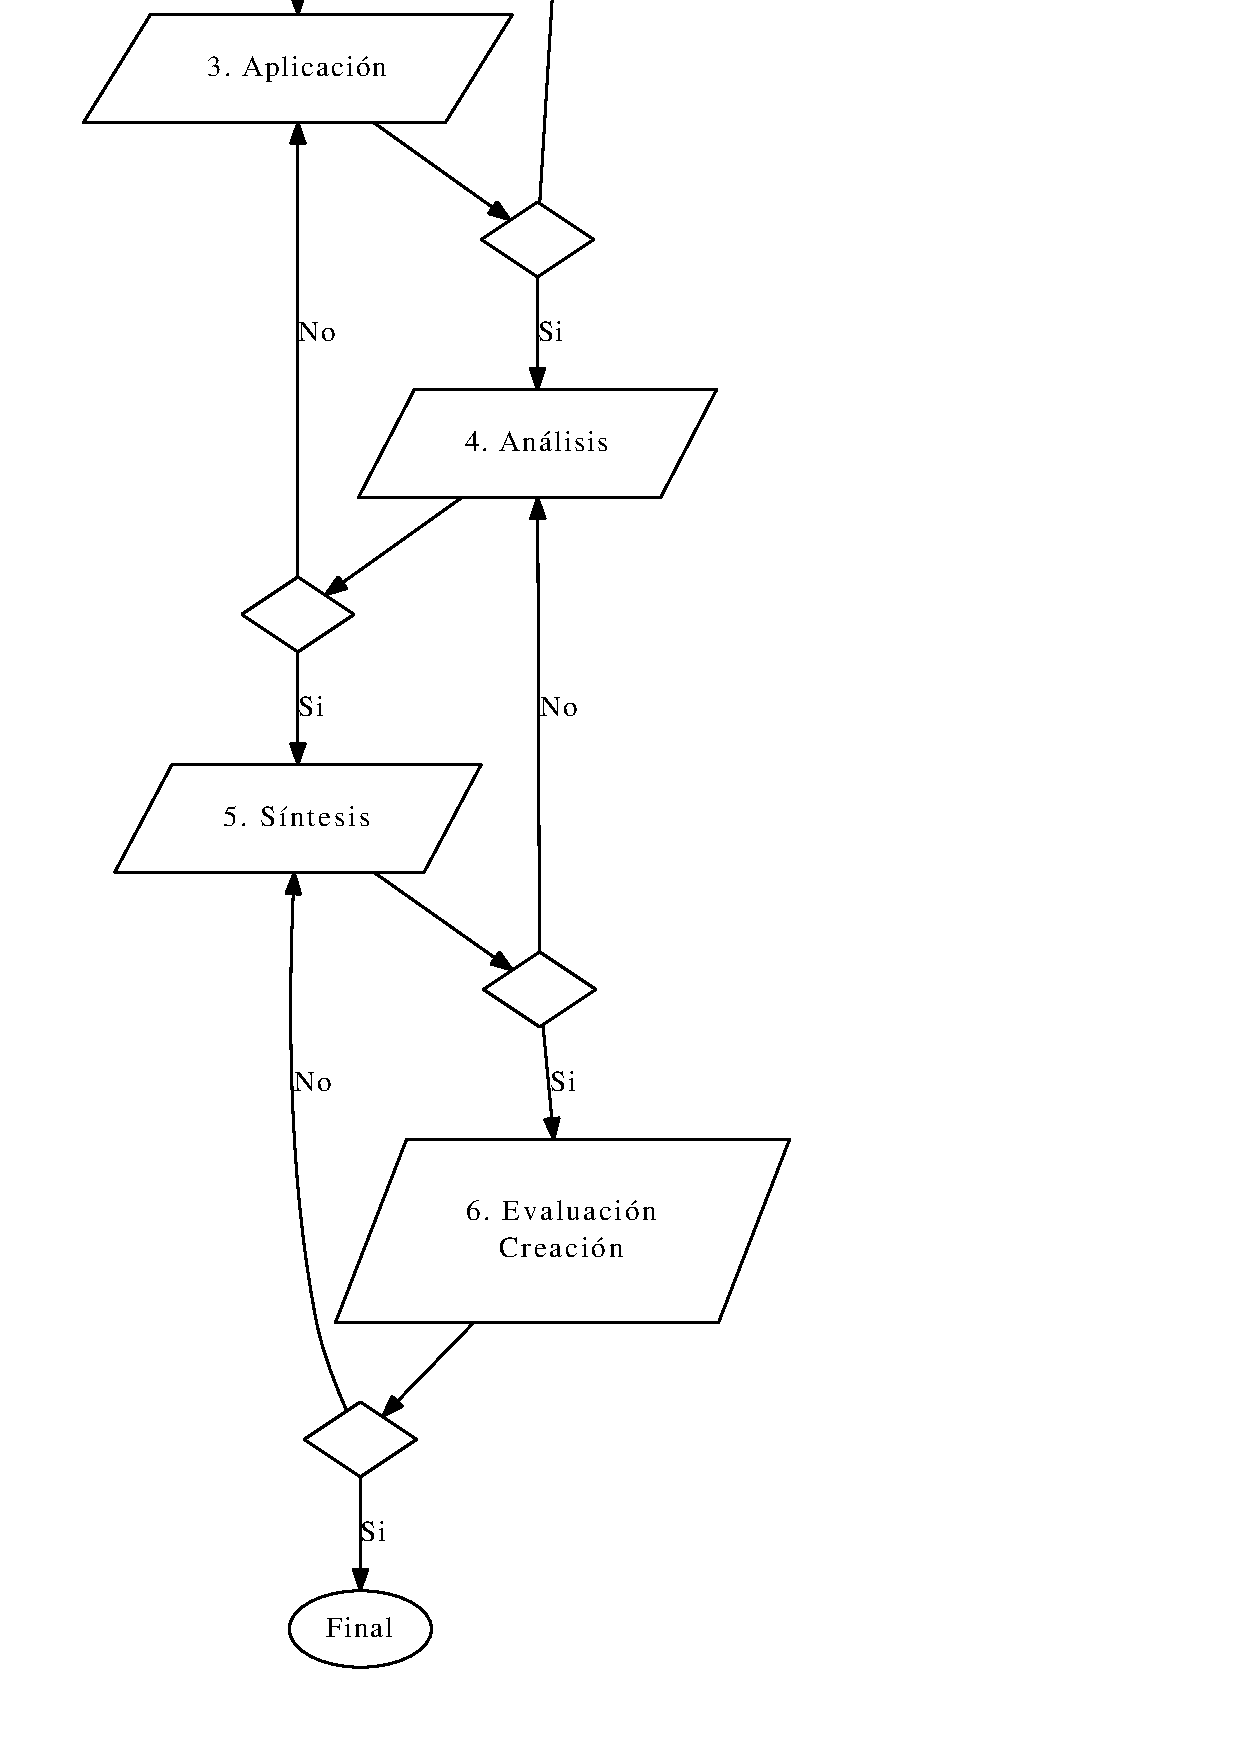
\includegraphics[height=10cm]{../fig/Bloom-sequence}}  & &
              \Cblur{\includegraphics[height=10cm]{../fig/Bloom}}     \\
              %{\captionsize Competencias por disciplina} &
              %{\captionsize Pir�mide del Aprendizaje} \\
        \end{tabularx}
}
{	
	~\\
% 	\vspace*{-0.7cm}
	\centering
	\newcommand{\bigstandard}{0.8\textwidth}
	\newcommand{\smallstandard}{0.41\textwidth}
	~\\
 	%\psframebox[framesep=3pt]{\includegraphics[width=0.84\textwidth]{../fig/X\currentarea-with-IS.eps}} \\
	\Cblur{\includegraphics[width=\bigstandard]{../fig/curves-\currentarea-with-CS.eps}} \\
	\vspace{0.2cm} 
	\color{white}{\captionsize \bf CS (\siglas) vs CS (ACM/IEEE-CS)}\vspace*{0.2cm}   \\
	\hrule \vspace{0.4cm} 	

	\begin{tabular}{cc}
                \Cblur{\includegraphics[width=\smallstandard]{../fig/curves-\currentarea-with-CE.eps}} &
                \Cblur{\includegraphics[width=\smallstandard]{../fig/curves-\currentarea-with-IS.eps}} \\
		\color{white}{\captionsize \bf CS (\siglas) vs CE (ACM/IEEE-CS)} & 
		\color{white}{\captionsize \bf CS (\siglas) vs IS (ACM/IEEE-CS)} 
	\end{tabular}
	\hrule \vspace{0.4cm}
	
	\begin{tabular}{cc}
                \Cblur{\includegraphics[width=\smallstandard]{../fig/curves-\currentarea-with-SE.eps}} &
		\Cblur{\includegraphics[width=\smallstandard]{../fig/curves-\currentarea-with-IT.eps}} \\
		\color{white}{\captionsize \bf CS (\siglas) vs SE (ACM/IEEE-CS)} & 
		\color{white}{\captionsize \bf CS (\siglas) vs IT (ACM/IEEE-CS)} 
 	\end{tabular}
	\hrule \vspace{0.4cm}
	
        \Cblur{\includegraphics[width=0.965\textwidth]{../fig/course-coding.eps}} \\
	\vspace*{0.2cm}
	\color{white}{\captionsize \bf Codificaci�n de cursos del �rea de Ciencia de la Computaci�n} \vspace*{0.2cm}\\ \hrule
	\vspace{0.4cm}
% 	\Cblur{\includegraphics[width=0.965\textwidth]{../fig/IS-course-number.eps}} \\
% 		\vspace*{0.2cm}
% 	\color{white}{\captionsize Codificaci�n de cursos del �rea de Sistemas de Informaci�n} \vspace*{0.2cm}\\ \hrule
% 	\hrule
%         \vspace{0.4cm}

	\Cblur{\includegraphics[width=0.965\textwidth]{../fig/\currentarea.eps}} \\
	\vspace*{0.2cm}\color{white}{\captionsize \bf Perfil internacional de CS} \vspace*{0.2cm}\\ \hrule
	\hrule \vspace{0.4cm}

	\begin{tabularx}{0.95\textwidth}{cX}
% 		\Cblur{\includegraphics[heigth=6.55cm]{../fig/pie-credits.eps}} &
% 		\Cblur{\includegraphics[heigth=6.55cm]{../fig/pie-by-levels.eps}} \\
		\Cblur{\includegraphics[height=6.55cm]{../fig/pie-credits.eps}} &
                \Cblur{\includegraphics[height=6.55cm]{../fig/pie-by-levels.eps}} \\
		\color{white}{\captionsize \bf Cr�ditos por �rea} & \color{white}{\captionsize \bf Cr�ditos por nivel}
 	\end{tabularx}
}

\begin{minipage}{\textwidth}
	{\bf \large \Copyrights}
\end{minipage}%

\end{document}
